\begin{figure}[H]
  \centering
  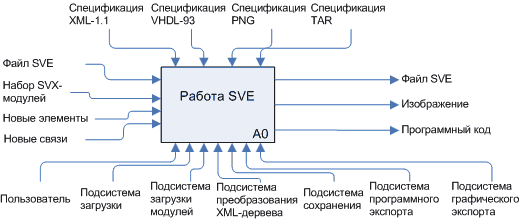
\includegraphics[width=0.7\textwidth]{diagrams/idef/a0-a.png}
  \caption{Контекстная диаграмма работы SVE}
  \label{fig:funcprot-1}
\end{figure}

На рисунке \ref{fig:funcprot-1} отражена структура системы и входящие в ее состав подсистемы.

\begin{figure}[H]
  \centering
  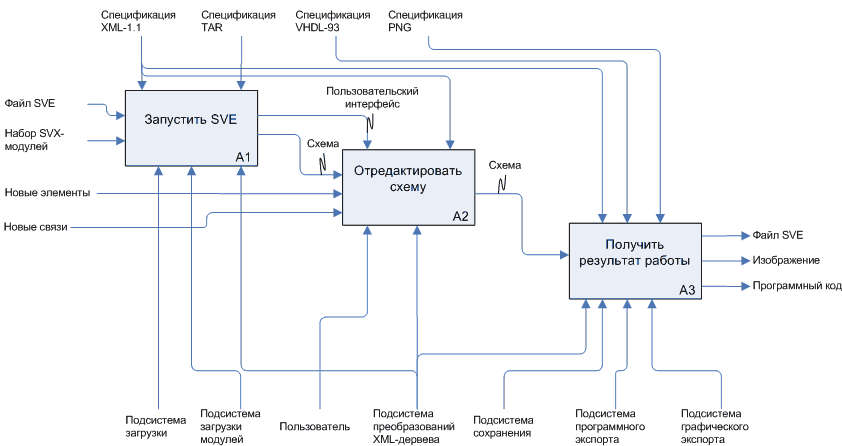
\includegraphics[width=1.0\textwidth]{diagrams/idef/a0-b.png}
  \caption{Декомпозиция контекстной диаграммы}
  \label{fig:funcprot-2}
\end{figure}

На рисунке \ref{fig:funcprot-2} показано, как задействованы подсистемы на различных этапах работы системы.

\begin{figure}[H]
  \centering
  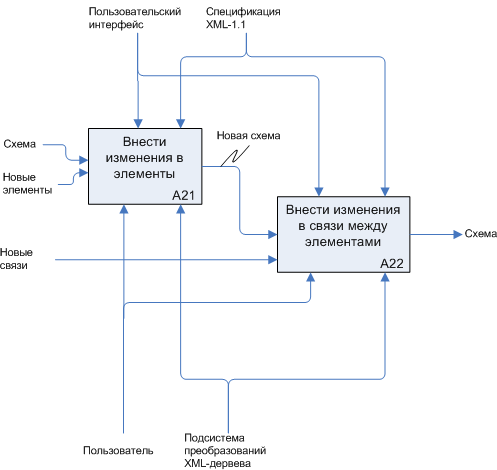
\includegraphics[width=0.8\textwidth]{diagrams/idef/a2-b.png}
  \caption{Декомпозиция процесса <<Отредактировать схему>>}
  \label{fig:funcprot-3}
\end{figure}

Из рисунка \ref{fig:funcprot-3} видно, что внесение изменений в узлы схемы ведет к пересчету связей в документе~--- так, например, перемещение узла ведет к перерисовке соединенных с ним связей.

\begin{figure}[H]
  \centering
  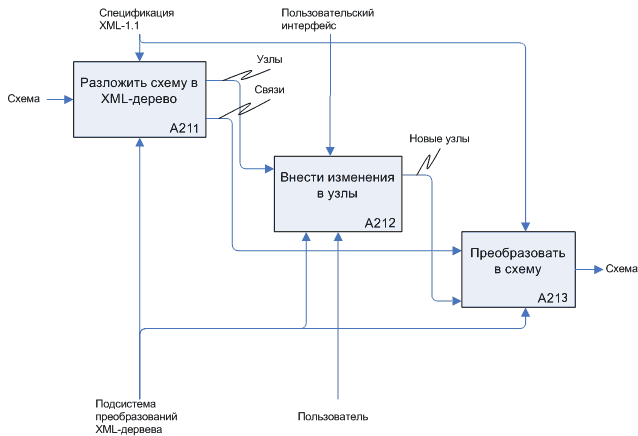
\includegraphics[width=0.95\textwidth]{diagrams/idef/a21-b.png}
  \caption{Декомпозиция процесса <<Внести изменения в элементы>>}
  \label{fig:funcprot-4}
\end{figure}

На рисунке \ref{fig:funcprot-4} показано, что редактирование элементов осуществляется по единому принципу~--- из XML-дерева документа извлекается соответствующий узел, его атрибуты подвергаются изменению, после чего узел помещается в дерево.

\begin{figure}[H]
  \centering
  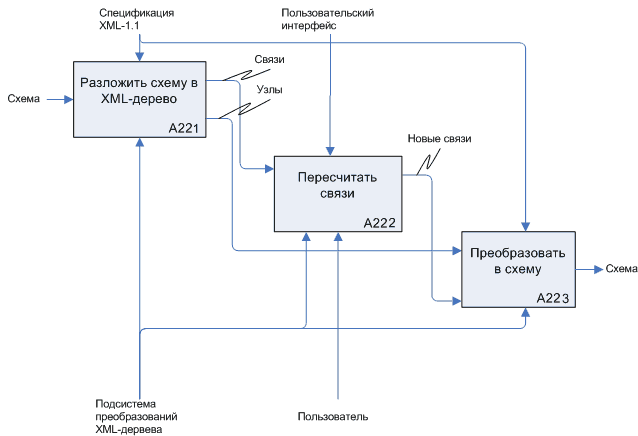
\includegraphics[width=0.95\textwidth]{diagrams/idef/a22-b.png}
  \caption{Декомпозиция процесса <<Внести изменения в связи>>}
  \label{fig:funcprot-5}
\end{figure}

Рисунок \ref{fig:funcprot-5} показывает, что редактирование связей ведется по аналогии с редактированием элементов, изложенным на рисунке \ref{fig:funcprot-4}.